\documentclass[crop,tikz,convert={outext=.svg,command=\unexpanded{pdf2svg \infile\space\outfile}},multi=false]{standalone}[2012/04/13]
%\usetikzlibrary{...}% tikz package already loaded by 'tikz' option

%%% Tikz libraries and definitions
\usetikzlibrary{intersections}
\usetikzlibrary{arrows}
\usetikzlibrary{calc}                 % coordinate calculations ($ n1 + (0:1cm) $)

% Common style for Simulink blocks.
\tikzstyle{block} = [rectangle, rounded corners, minimum width=3cm, minimum height=0.8cm,text centered, thick, draw=black]
% Common style for connectors. 
\tikzstyle{arrow} = [->,>=stealth',font=\scriptsize,rounded corners]

% Some distances to share between figures.
\newcommand{\shift}{0.28cm}
\newcommand{\bigshift}{1cm}




\begin{document}

  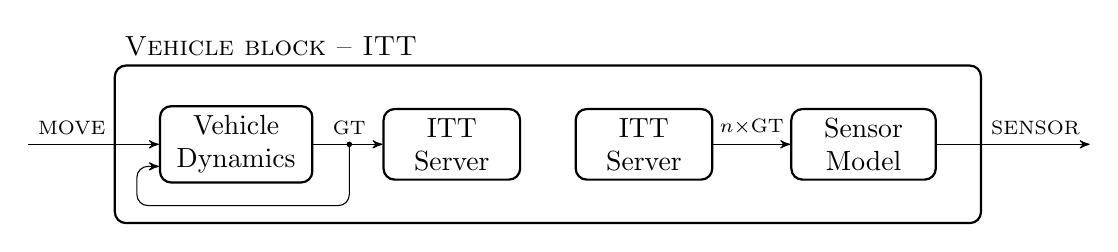
\begin{tikzpicture}[node distance=2cm]
  
  %\draw[help lines] (-2,-2) grid (2,2);
  \coordinate (top) at (0,1);
  \coordinate (left) at (-2,0);
  \coordinate (bottom) at (0,-1);
  \coordinate (right) at (9,0);
  \coordinate (vehicleModel) at ([xshift=2*\shift]left);
  \coordinate (sensorModel) at ([xshift=-2*\shift]right);
  \coordinate (leftMux) at ([xshift=\shift+4*\bigshift]left);
  \coordinate (rightMux) at ([xshift=-\shift-4*\bigshift]right);


  % Whole block
  \draw (top -| left) [block] rectangle (bottom -| right);

  % Block title
  \node [anchor=south west] (Blockname) at (top -| left) {\textsc{Vehicle block -- ITT}};


  % Vehicle Model
  \node [block, anchor=west, minimum width=1.5cm, text width=1.7cm] (vehicleModelBlock) at (vehicleModel) {Vehicle Dynamics};


  % Sensor Model
  \node [block, anchor=east, minimum width=1.5cm, text width=1.6cm] (sensorModelBlock) at (sensorModel) {Sensor Model};


  % Left MUX
  \node [block, minimum width=1cm, text width=1.5cm] (udpsend) at (leftMux) {ITT Server};


  % Right MUX
  \node [block, minimum width=1cm, text width=1.5cm] (udpreceive) at (rightMux) {ITT Server};


  % GT feedback
  \draw [arrow] (vehicleModelBlock) -- node [anchor=south east,name=GT,pos=0.9] {GT} (udpsend);
  \fill (GT|-vehicleModelBlock) circle [radius=1pt];
  \draw [arrow] (GT|-vehicleModelBlock) |- ([yshift=-\shift,xshift=-\shift]vehicleModelBlock.south west) |- ([yshift=-\shift]vehicleModelBlock.west);

  % n x GT
  \draw [arrow] (udpreceive) -- node [anchor=south] {$n \times$GT} (sensorModelBlock);

  % Input
  \draw [arrow] ([xshift=-1.1*\bigshift]left) node [anchor=south west] {MOVE} -- (vehicleModel);

  % Output
  \draw [arrow] (sensorModel) -- node [anchor=south east,at end] {SENSOR}([xshift=1.1*\bigshift+\shift]right);


  \end{tikzpicture}

\end{document}
